\section{Электрофорез (8 сентября)}
\subsection{Определение концентрации пробы 4}
Предполагалось, что в пробе 4 содержится суспензия альдолазы.
Чтобы исследовать пробу 4 методом электрофореза,
требуется знать примерную концентрацию белка в пробе.
Для этого провели ещё одно спектрофотометрическое определение концентрации.

Было отобрано 10 µl пробы и помещено в кювету объемом 2 ml.
Разведение составило 201 раз.

$$ A_{260} = 0.110 $$
$$ A_{280} = 0.148 $$

По формуле Калькара
$$ c = N (1.45 A_{280} - 0.74 A_{260} = 201 (1.45 \cdot 0.148 - 0.74 \cdot 0.110) = 26.8 \text{mg/ml}$$

Учитывая, что проба 4 считается очищенной от нуклеотидов и остальных белков,
можно применить следующую формулу:
$$ c = N \frac{A_{280}}{\epsilon l} = 201 \frac{0.148}{0.91 \cdot 1} = 32.7 \text{mg/ml}$$

Таким образом, концентрацию альдолазы в пробе 4 будем считать 32.7 mg/ml.

\subsection{Определение концентрации пробы 2}
Так как значения концентрации пробы 2 получились довольно разными,
было проведено повторное определение концентрации пробы 2 спектрофотометрическим методом.

Было отобрано 80 µl пробы и помещено в кювету объемом 2 ml.
Разведение составило 26 раз.

$$ A_{260} = 0.526 $$
$$ A_{280} = 0.343 $$

По формуле Калькара
$$ c = N (1.45 A_{280} - 0.74 A_{260} = 26 (1.45 \cdot 0.343 - 0.74 \cdot 0.526) = 2.8 \text{mg/ml}$$

\subsection{Исходные концентрации проб}
После рассмотрения концентраций проб, полученных спектрофотометрическим методом
и методом Брэдфорд, было обнаружено, что точность концентрации пробы 2 вызывает
сомнения.

Значения концентрации пробы 3, полученные обоими методами, почти совпали (6 mg/ml).
Концентрация пробы 1 принята за 15.6 mg/ml.
Концентрация пробы 2 должна быть меньше концентрации пробы 1
(уже потому, что объем, из которого отбиралась проба 1,
меньше объема, из которого отбиралась проба 2).
В то же время, концентрация пробы 2 должна быть больше концентрации пробы 3,
так как проба 3 отбиралась из раствора, из которого была удалена альдолаза.
Учитывая эти соображения, решили, что концентрация пробы 2 равна 10.8 mg/ml.

\subsection{Разбавление белковых проб}
Известно, что для использования пробы в электрофорезе концентрация
белка должна быть примерно 0.5 mg/ml.
Объем образца для электрофореза: 200 µl.
Было решено сначала разбавить все пробы в 5 раз, после чего
отобрать из них объем, необходимый для электрофореза.

Чтобы получить образец с концентрацией 0.5 mg/ml,
из раствора, полученного разбавлением пробы в 5 раз,
необходимо отобрать
$$ V = N \frac{C_2 V_2}{C_1} = 5 \frac{0.5 \text{mg/ml} \cdot 0.2 \text{ml}}{C_1} = \frac{0.5}{C_1} \text{[ml]} $$
где $C_1$ -- концентрация белка в пробе.

Рассчитаем объемы, которые нужно отбирать из разбавленных в 5 раз проб:

\begin{tabular}{|c|c|c|}
\hline
Проба & $C_1$ [mg/ml] & $V$ [µl] \\
1 & 15.6  & 32.05 \\
2 & 10.8  & 46.3  \\
3 & 6.2   & 80.65 \\
4 & 32.7  & 18.7  \\
\hline
\end{tabular}

\subsection{Приготовление образцов для электрофореза}
4-х кратный буфер для образцов (SB) был выдан преподавателем.
Для получения однократного буфера, 4-х кратных буфер был разбавлен в 4 раза.
В 1 мл SB было добавлено 50 µl меркаптоэтанола,
концентрация меркаптоэтанола в полученном буфере 5\%.
Для получения образцов для электрофореза сначала добавляли воду,
затем пробу белка, разведенную в 5 раз, затем 50 µl SB.

\begin{tabular}{|c|c|c|c|}
\hline
Проба & \ce{H20} & Проба/5 & SB \\
1 & 118 & 32   & 50 \\
2 & 104 & 46   & 50 \\
3 &  70 & 80   & 50 \\
4 & 131 & 18.7 & 50 \\
\hline
\end{tabular}

\subsection{Маркеры для электрофореза}
\begin{enumerate}
\item Phosphorilase B, 97 kDa
\item BSA, 66.2 kDa
\item Ovalbumin, 45 kDa
\item Carbonie anhydrase, 31 kDa
\item Trypsin inhibitor, 21.5 kDa
\item Lysozime, 14.4 kDa
\end{enumerate}
Оптимум нанесения: 3--5 µl на дорожку.
Хранение при -20\celsius.

\subsection{Проведение электрофореза}
В 10 лунок геля были нанесены образцы:
\begin{enumerate}
\item маркер
\item проба 1 (8 µl, 4 µg)
\item проба 2 (8 µl, 4 µg)
\item проба 3 (8 µl, 4 µg)
\item проба 4 (8 µl, 4 µg)
\item пустая
\item проба 1 (16 µl, 8 µg)
\item проба 2 (16 µl, 8 µg)
\item проба 3 (16 µl, 8 µg)
\item проба 4 (16 µl, 8 µg)
\end{enumerate}

Параметры электрофореза: 20 mA, 400 V.

\subsection{Результаты электрофореза}
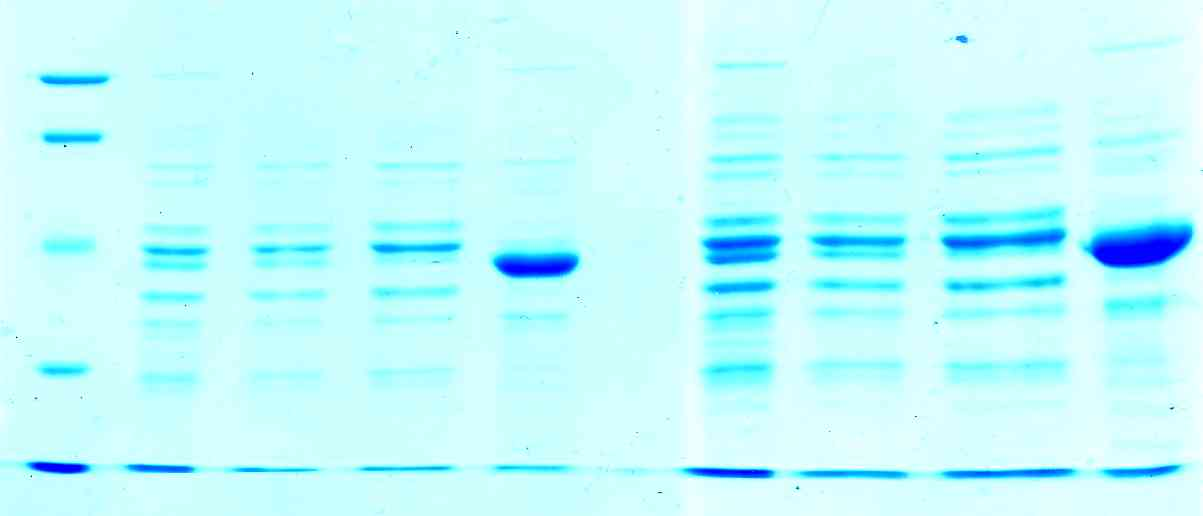
\includegraphics[width=\linewidth]{ef.jpg}

\emph{Вывод}: последняя стадия эффективно отделила альдолазу.

